\documentclass[12pt]{article}
\usepackage[a4paper, total={6.5in, 8.5in}]{geometry}
\usepackage[english]{babel}
\usepackage{graphicx}
\usepackage[autostyle, english = american]{csquotes}
\MakeOuterQuote{"}
\usepackage{xargs}
\usepackage{longtable}
\usepackage{amsmath,amssymb}
\usepackage{tabularx}
\usepackage{hyperref}
\usepackage[dvipsnames]{xcolor}
\hypersetup{
    colorlinks=true,
    linkcolor=black,
    filecolor=magenta,      
    urlcolor=cyan,
    pdftitle={Overleaf Example},
    pdfpagemode=FullScreen,
    }
    
\usepackage{svg}

\newcolumntype{R}[1]{>{\raggedleft\arraybackslash}p{#1}}
\newcolumntype{L}[1]{>{\raggedright\arraybackslash}p{#1}}
%\newcolumntype{L}[1]{>{\raggedright\let\newline\\\arraybackslash\hspace{0pt}}p{#1}}

\newcounter{mycounter}
\newcommand{\rowlabel}[1]{\refstepcounter{mycounter} \label{#1}}

\begin{document}
	
	\title{\hfill\\\hfill\\\Huge Rulebook}
	\author{Michal Horanský}
	\maketitle
	
	\begin{center}
	\vspace*{-10.5cm}\hspace*{1.1cm}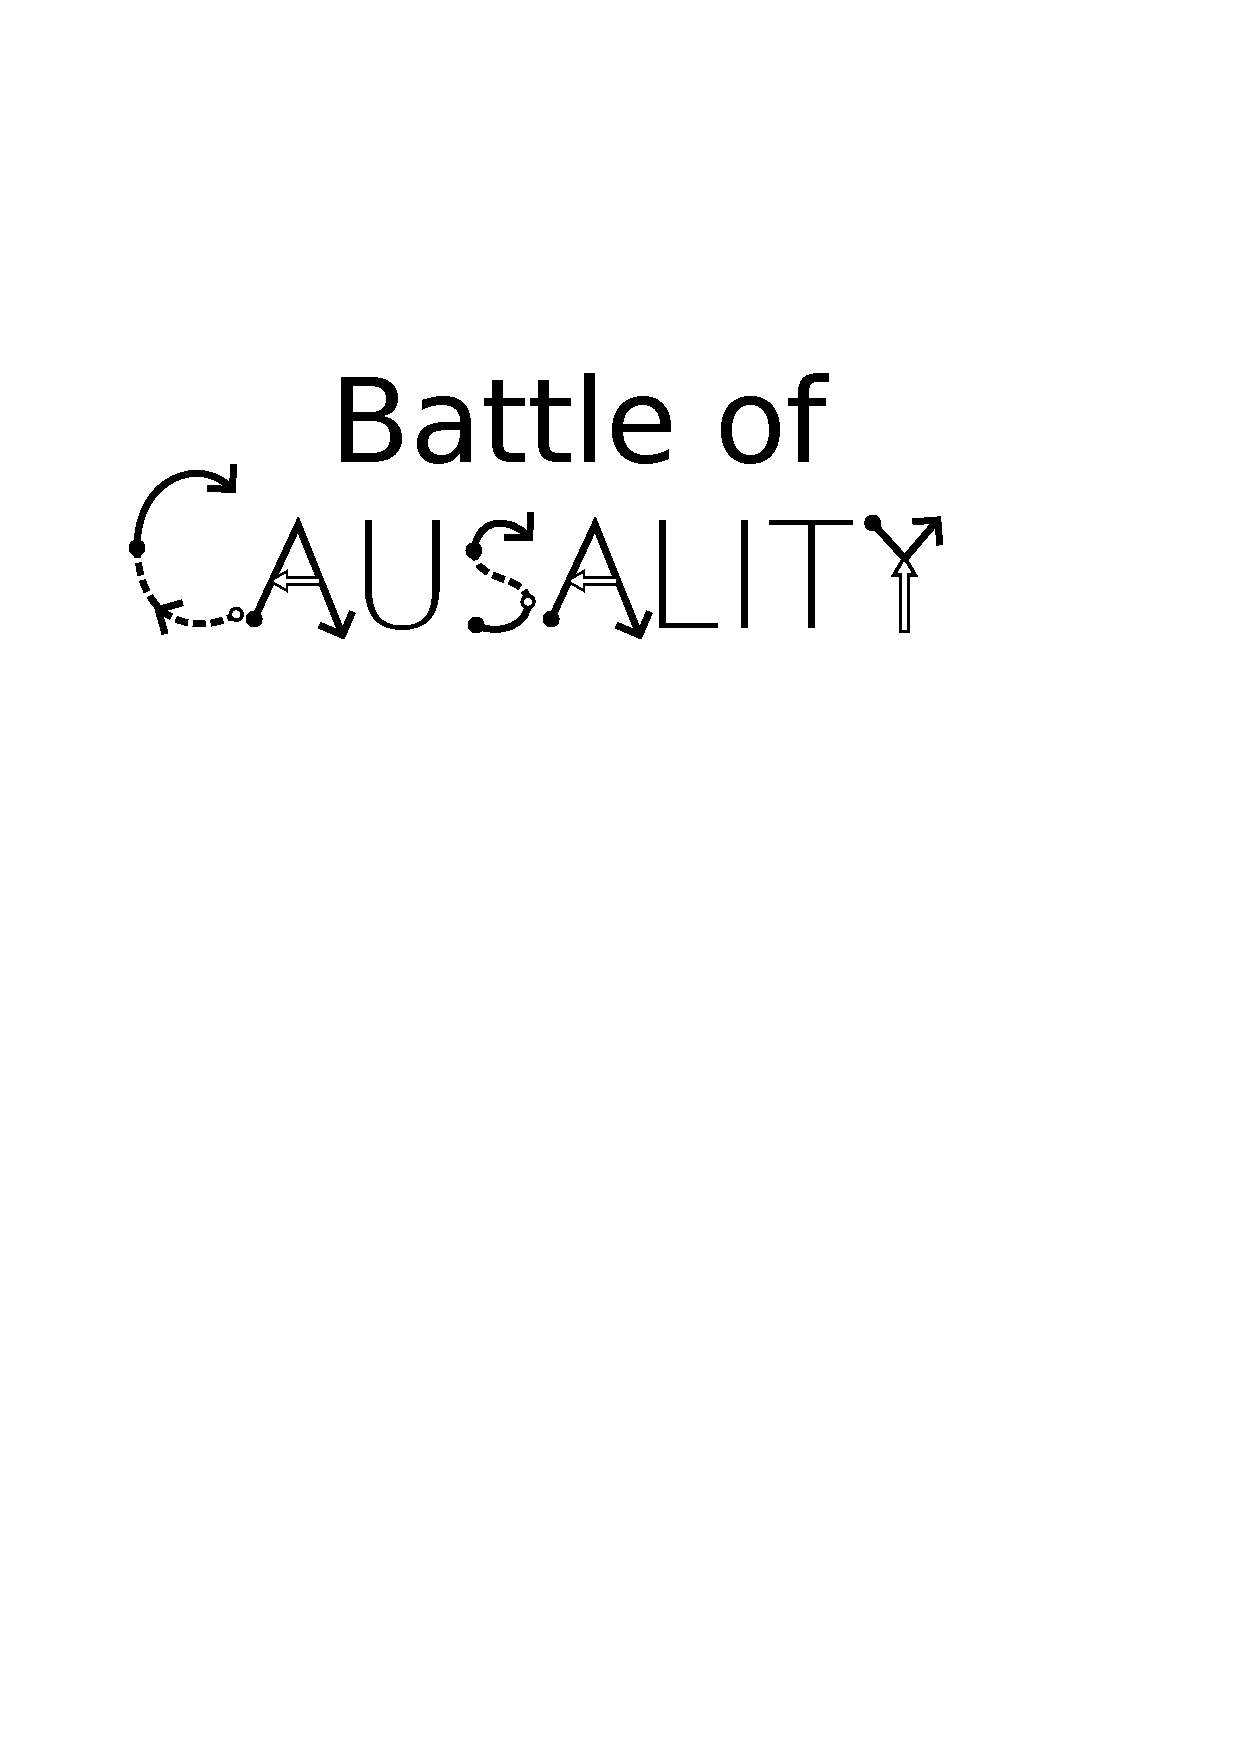
\includegraphics[scale=0.5]{images/BoC_logo}\vspace*{-4.5cm}
	\end{center}
	
	\tableofcontents
	
	\section{Introduction}
	\textit{Battle of Causality} is a turn-based digital strategy board game about time-travel. To address the elephant in the room which typically barges in at this point and loudly asks: "So how is it different from \textit{5D Chess With Multiverse Time Travel}?" In \textit{5D Chess With Multiverse Time Travel}, you cannot "change the past" in a way that affects a board configuration which has already been reached--attempting to do so creates a new timeline, which is a neat resolution of the ontological paradox. \textit{Battle of Causality} tackles time-travel in a completely different way, utilising the Novikov self-consistency principle. A stone may travel back in time, but such an action only occurs if it can be "justified" by the player's actions, i.e. any caused effects don't contradict their initial causes. In short, there is a single timeline which hosts an increasing number of tangled world lines, where effect may precede cause, and the growing danger of a paradox looms ever-present.
	
	\subsection{Setting}
	\begin{quote}
	\textit{Cover blown, those few souls made their mad dash towards the enemy's fragile heart, trapped impossibly between the rattle of weaponry and the clock rapidly bleeding time. Yet, in the eleventh hour, they found the rivers of blood running upstream, they witnessed the intangible skein wound from all their struggle undoing itself, until all this impossible movement dissolved into anticipation. Now they face the same odds, and the same struggle, but the scales have been tipped. Now it is they who observe and are not observed, until the moment arises when they tap the shoulder of the man turning his back to face them. Seeing pictures from their pasts running past, object and image converge and the mirror breaks again and again. We found in that point of eternal return the very source of struggle itself: anticipation.}
	\end{quote}
	Two players, $A$ and $B$, face each other in a competitive battle over the board. Each player controls an army of stones with diverse specialisations and abilities. Commandeering their stones as time progresses, the players attempt to destroy the opponent's army to clear the way for capturing all the strategically significant points. However, time runs short, and after a few turns, there is nowehere to move anymore. The game, however, continues: the stones can be commanded not just to move in space, but also to jump back in time. These new versions of the old stones share the board space with their previous versions, which follow the established routes already known to the players. However, should a stone travel back in time and obstruct the path of its old self, history becomes malleable. And so the players can control an ever-growing and ever-changing army of many mirror images of a handful of stones, which constantly rewrite their own history. However, be careful not to perform an action which contradicts itself, or you might find yourself trapped in a paradox...
	
	\subsection{Goal of the game}
	
	The board houses a few special squares called bases. Each base has an allegiance: it can belong to either player, or be neutral. Players can capture bases by visiting them with their stones, which changes the base's allegiance to the player's faction until it is captured by their opponent. The goal of the game is to make sure that all the bases on the board belong to you.
	
	\section{How to play}
	The board consists of squares placed along three axes: horizontal position $x$, vertical position $y$, and time $t$. Time is, of course, special, as the state of the squares at a particular time is directly inferred from the state of the squares at a lower time. The collection of squares at a specified time is called a time-slice, and can be thought of as the temporal equivalent of a rank or a file in classical chess. The dimension of the board along the time axis is called the time cap: the whole game takes place in a time interval of length restricted by this time cap.
	
	\begin{figure}[h]
\begin{center}

    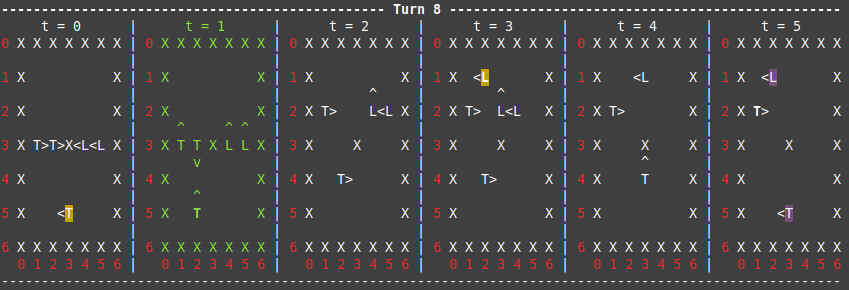
\includegraphics[width=0.9\textwidth]{images/diag_game_example}
 \caption{This is an example of a game in-progress. This board has a time cap of $6$, so there are six time-slices organized from earliest to latest, left to right. Player $A$ and player $B$'s stones are labelled T and L, respectively. The game is already on turn $8$, which for this time cap corresponds to round $2$ and active time-slice $t=1$. In the active time-slice, player $A$ has only one causally free stone at $(x=2, y=5)$ which they can command in this turn, and player $B$ will not be able to place down any flags until turn $10$, where they have a causally free stone at $(x=2, y=1)$.}\label{fig:game example}
\end{center}
\end{figure}
	
	The game is played in rounds, where every round consists of a number of turns equal to the time cap. In each round, the players look at the first time-slice in the first turn, then the second time-slice in the second turn etc, until they reach the time cap. In each turn, both players simultaneously place down flags in the active time-slice, which are essentially commands for their stones, and after each turn, those flags are translated into actions performed by the stones, which determine the state of the next time-slice.
	
	At the end of each round, a procedure called \textbf{canonisation} is performed, which resolves everything to do with time-travel and sets the stage for the first time-slice of the next round. At this moment, it is also checked if the end-of-game conditions have been satisfied.
	
	An important thing to note is that a flag being placed for a stone at a time-slice $t$ affects the stone "in-between" this and the next time-slice, and the consequences of that action showly on in the next time-slice $t+1$.
	
	\subsection{Stone trajectories and flag placement}\label{sec:trajectories}
	Every stone placed on the board has a unique flag called the \textbf{progenitor} which, if active, places it onto a specific position. From the corresponding time onwards, the stone checks the square it stands on in each time-slice for flags which can be activated (see Sec. \ref{sec:flag activation conditions}). Activating a flag determines the stone's initial placement in the next time-slice, and after all flags in this time-slice are dealt with, this initial placement is changed into the canonical placement by resolving all conflicts (see Sec. \ref{sec:spatial conflict resolution}). If the stone follows a flag which removes it from a board, is destroyed, or becomes causally free, it is not placed into the next time-slice, and its trajectory ends.
	
	\begin{figure}[h]
\begin{center}

    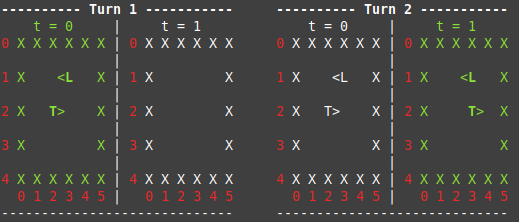
\includegraphics[width=0.6\textwidth]{images/diag_placing_flags}
 \caption{This is a board with a time cap of $2$. In the first turn of the round, two stones are placed on setup, but since they are causally free (see Sec. \ref{sec:causal freedom}), they are not present in time-slice $t=1$. In the first turn, player $A$ tells their tank to move forward by one square, and player $B$ tells their tank to wait. Hence, in second turn, the two stones are placed in both time-slices, being causally free only in time-slice $t=1$.}\label{fig:placing flags}
\end{center}
\end{figure}

	It is important to note that the game is \textbf{totally deterministic}. In other words, specifying the flags players placed on each turn up to turn $T$ allows us to unequivocally ascertain the state of the board on turn $1$, turn $2\dots$ all the way to turn $T$.
	
	\subsubsection{Causal freedom and the comb rule}\label{sec:causal freedom}
	If a stone reaches a position at which there is no flag which it can follow, the stone becomes \textbf{causally free}. This means that we don't know what the stone does between this and the next time-slice, and so it isn't yet placed in the next time-slice. However, when a flag is placed for this stone at the point of its causal freedom, it gets "locked" into the specified action and can be placed into the next time-slice, where (if not destroyed) it is causally free and can be commanded again.
	
	Now we understand the structure of the game as divided into rounds and turns: the turns progress through every time-slice "sweeping up" causally free stones, propagating their trajectories to the point of removal from the board or the time cap. Then, when the end of the round is reached, any progenitor flag, including the newly placed time-jumps, can be set as active, which in turn creates new causally free stones sprinkled over the board, and a new round of "sweeping" may begin again.
	
	The \textbf{comb rule} states that within a round, the past is always known. In other words, in a turn where time-slice $t$ is active, there cannot be any causally free stones in time-slices $1, 2\dots t-1$. This mean that the players have to command \textit{all} of their causally free stones at $t$, with the only exception to this being the final time-slice of the round, where stones are allowed to be left as causally free, since there is no later time at which their past would have to be known (see Fig. \ref{fig:comb rule}).
	
	\begin{figure}[h]
\begin{center}

    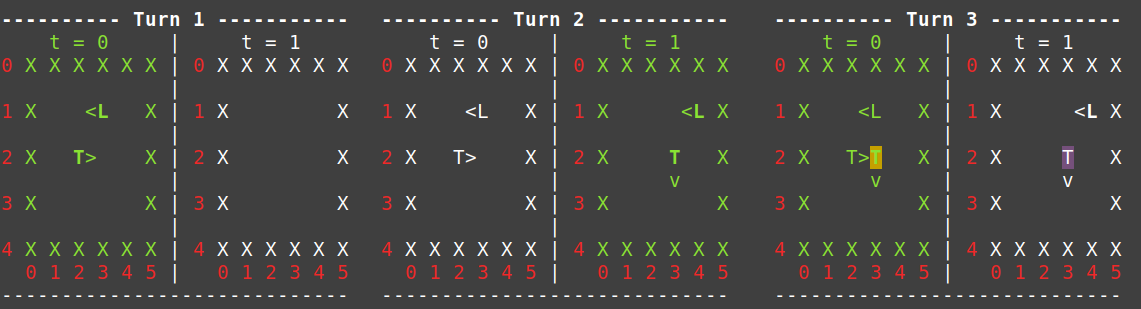
\includegraphics[width=0.9\textwidth]{images/diag_rule_of_combing}
 \caption{This is a board with a time cap of $2$. Causally free stones are printed in \textbf{bold}. In the first turn, both players have to command their stones due to the comb rule. In the second turn, player $A$ commands their tank T to jump back into $t=0$, but player $B$ doesn't place any flags for their tank L, leaving it causally free at $t=1$. This is why in the next round in turn 3, only player $A$ has a causally free stone to command in the active time-slice.}\label{fig:comb rule}
\end{center}
\end{figure}
	
	This shows the structure of the game analogous to combing one's hair: a tangled mess of unknown worldlines is laid out at the beginning of each round, and then a comb is brought down in the forward direction, leaving the hair behind straightened out, only to be lifted after reaching the neck and repeating the process over and over. The comb rule then relates the fact that a comb always moves in one direction only.
	
	\subsubsection{Interference}
	An important term to be familiar with is \textbf{interference}. The philosophy the game follows is that trajectories once laid out will play out again and again, unless their actors are interacted with by stones sharing the same time, but still remaining causally free due to being placed into the same time later in the game. If a stone which would not normally become causally free in a specific time-slice has its path obstructed or is in another way prevented from reaching the next flag leading it along its trajectory, that stone once again becomes causally free in that time-slice. In short, the more interference the players can cause among their stones, the more control over them they can gain.
	
	
	\subsubsection{Preventing amnesia}\label{sec:flag activation conditions}
	Firstly, a flag (which is not a progenitor) associated with a stone requires that stone to be present at its position in order to be activated. However, this is a necessary, but not a sufficient condition. Consider the situation outlined in Fig. \ref{fig:amnesia}.
	
\begin{figure}[h]
\begin{center}
    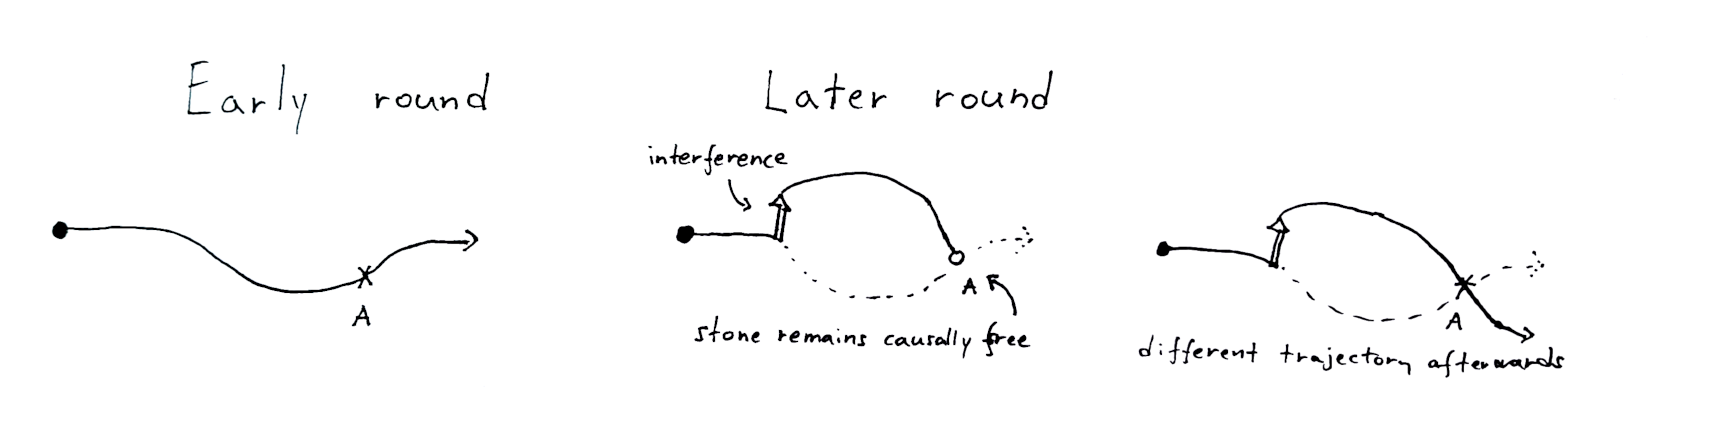
\includegraphics[width=1\textwidth]{images/diag_amnesia}
 \caption{A stone follows a certain trajectory in an early round, where it reaches position $A$ and an associated flag is placed for it at that position. In a later round, the stone's trajectory is broken by interference preceding $A$, and the stone takes a different trajectory. However, the new trajectory also reaches point $A$. Now: at $A$, a flag already exists for this stone in this later round. Nevertheless, this flag does \textit{not} get activated, because it was placed in an earlier round than the flags the stone already followed along this later trajectory. The stone doesn't "forget" the interference, and it doesn't slip into an old trajectory if given the chance. The trajectory from the earlier round may still get realised in an even later round if the interference effect disappears from the canon.}\label{fig:amnesia}
\end{center}
\end{figure}
	
	
	Therefore, the general rule is as follows: If multiple active flags associated with a stone at a specific position exist at that position, the flag placed in the \textit{earliest round which is not earlier than the last flag the stone followed in the previous time-slice} is activated.
	
	\subsubsection{Order of flag execution}
	Once all flags have been placed for this turn, the game calculates the state of the board for the next turn. It does this by going from the first to the last time-slice, always taking the flags in the previous time-slice to determine the state of this time-slice. This process can be broken down into four parts:
	\begin{enumerate}
		\item The movement flags placed on the previous time-slice and progenitor flags associated with this time-slice are executed, propagating the stones into this time-slice, in general into conflicting positions.
		\item The spatial conflicts are resolved, and the state of this time-slice is conflict-free.
		\item The stone actions activated in the previous time-slice, such as attacks, and board events such as explosions of bombs and tagscreens, are resolved now. Since these can only remove stones from the board, but not push them, the time-slice remains without conflict.
		\item Finally, the allegiance of each base changes to the faction of the occupying stone, if there is one. The time-slice state is now canonical.
	\end{enumerate}
	Note that, within each turn, there is no order imposed upon the players--rather, all of the commands they submitted are performed simultaneously! An important part of the game is also that players choose their actions in a given turn without seeing what the other player is considering to do, only learning of each other's actions after the turn ends.
	
	\subsection{Spatial movement and attacking}
	The simplest action a stone typically performs is moving spatially. Different stone types move in different ways, which are described in Sec. \ref{sec:stone types}. Each stone type has two parameters which partially describe its interaction with other stones and its control scheme with regard to spatial movement:
	\begin{itemize}
	\item \textbf{Orientability}: If a stone is orientable, it is described not only by its spatial position, but also the direction it is facing, referred to as its "azimuth". Typically, the azimuth of a stone is one of the four cardinal directions. The azimuth of an orientable stone determines the direction of its movement and attacks.
	\item \textbf{Opposability}: The full extent of this property is described in Sec. \ref{sec:spatial conflict resolution}, but to put it simply, \textbf{unopposable} stones jump over other stones when moving, while \textbf{opposable} stones push other stones along the direction of their movement.
	\end{itemize}
	The most important rule of movement in \textit{Battle of Causality} is: two stones cannot occupy the same square! If two stones do end up on the same square after the placed commands are executed, the game rearranges their positions following a process called spatial conflict resolution (see Sec. \ref{sec:spatial conflict resolution}) until the time-slice is conflict-free. A \textbf{conflict} is an occurence on the board where either a stone occupies an unavailable square, such as a wall, or two or more stones occuppy the same square. The game prevents conflicts in two ways:
	\begin{itemize}
	\item "Soft" prevention: the player will not be allowed to place down a flag which would command their stone into a permanent, static obstacle (i.e. an unavailable square).
	\item "Hard" prevention: after all movement commands are executed, spatial conflict resolution assures the next time-slice to be conflict-free.
	\end{itemize}
	
	\subsubsection{Spatial conflict resolution}\label{sec:spatial conflict resolution}
	The conflict resolution routine represents the physicality of the stones. Even though the routine may revert the spatial movement of a stone, note that if the stone also changed its azimuth, this azimuth change does not revert. Its core philosophy is that the stones are "sokoban-like", and hence can be pushed by movement of other stones. The rules for conflict resolution are applied in order as follows:
	\begin{enumerate}
		\item "Sokoban push": For every square occupied by exactly two stones, if one of these stones occupied the same square in the previous time-slice, it will be pushed in the direction of the other stone's approach. This will not occur if
		\begin{itemize}
			\item the other stone did not move onto this square from the previous time-slice spatially, but rather was placed here by a progenitor flag, e.g. through a time-jump-in, or
			\item the square onto which the stone would be pushed is unavailable or occupied (much like in Sokoban, one cannot push two stones with one move), or
			\item the other stone is not opposable.
		\end{itemize}
		\item "Opposition": For every opposable stone, if it moved from position A to position B and there exists another opposable stone which moved from position B to position A, both stones are returned to their original position.
		\item "Pyrotechnics" : Explosive stones destroy all stones which share their square, and, optionally, themselves.
		\item "Impasse": Now, for every square occupied by more than one stone, all the stones on this square which have \textbf{not} been placed on the board in this time-slice (i.e. they are present in the previous time-slice) are moved back to the square which they occupied in the previous time-slice, as well as the stones they pushed through the "sokoban push" rule. This rule chains, and is applied repeatedly until all stones which are still placed on squares which are occupied by more than one stone have already been moved by this rule.
		\item "Explosion": Finally, for every square occupied by more than one stone, all stones on this square are removed from the board.
	\end{enumerate}
	Notice the order of these rules. We see that sokoban pushes only happen to stones which have not moved between this and the previous time-slice, or have been placed onto the board, but rather chose a stationary action, such as "wait", "rotate", "attack" etc. Notably, two stones moving onto the same square, be it in opposing or perpendicular directions, are returned back onto their original squares due to the "impasse" rule. This means that no stone has priority in movement. Also, if a stone time-jumps-in at time $t$ on the same square a stone moves onto from time-slice $t-1$, the spatial movement of the second stone is blocked. Hence, opening time portals are treated as momentary blockades.% Finally, since the "sokoban push" rule doesn't apply if the waiting stone would be pushed onto an occupied square, this means that sokoban-like movement does have a lower priority than regular movement (you can think of this as the fact stones are "slowed down" by pushing a stone in front of them). For an example, see Fig. \ref{fig:scr_1}.
	
	%\begin{figure}[h]
%\begin{center}
    %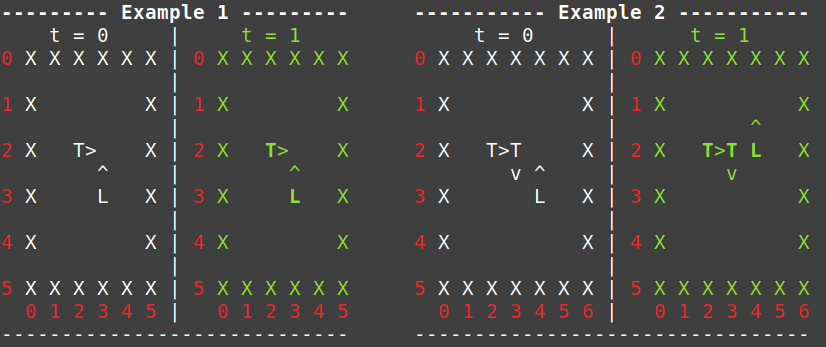
\includegraphics[width=0.6\textwidth]{images/diag_scr_1}
 %\caption{In Example 1, both stones attempt to move forwards, forming an impasse and halting. In Example 2, however, the tank at $x=2,y=2$ now also attempts to sokoban-push another tank (which is performing a waiting action), which does \textbf{not} result in an impasse, and the tank at $x=4,y=3$ successfully moves, demonstrating the de facto priority unburdened movement has over sokoban pushing.}\label{fig:scr_1}
%\end{center}
%\end{figure}
	
	The second rule "opposition" is a simple manifestation that moving stones cannot simply phase through each other if moving in opposite directions, unless they are stones which "jump" over others (i.e. unopposable stones).
	
	The third rule "pyrotechnics" simply designates the proper time at which certain stone actions are performed, such as the activation of mines when being stepped on, or the offensive move of a wildcard-type stone (see Sec. \ref{sec:stone types}). Its position after sokoban pushing and opposition, but before impasse, is deliberate, as stones can be pushed onto mines or into the wildcard's captures, and if two or more stones attempt to move onto a square with a mine, the fact that the impasse rule would block their movement does not save them (see example in Fig. \ref{fig:scr_1}).
	
	\begin{figure}[h]
\begin{center}
   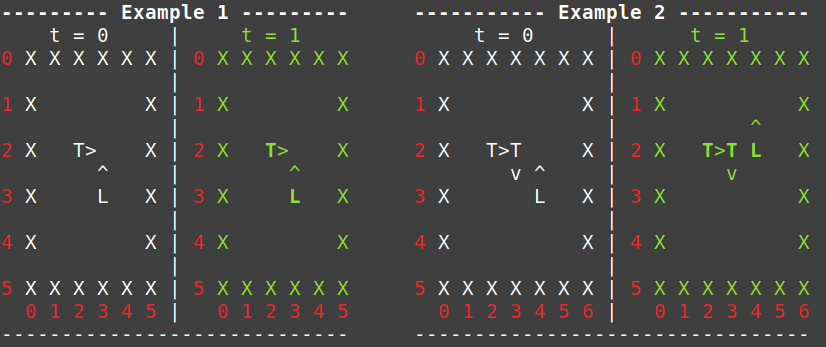
\includegraphics[width=0.4\textwidth]{images/diag_scr_1}
 \caption{In this example, both tanks move forward, sokoban-pushing the sniper, which would normally form an impasse with the bombardier moving upwards. However, a wildcard moves onto the same square, destroying the sniper and the bombardier, but not blocking the tanks' advance.}\label{fig:scr_1}
\end{center}
\end{figure}
	
	Note that the fourth rule "impasse" does chain. Thus, if multiple moving stones form a "promenade", each moving onto the previous stone's square of origin, a single "impasse" event at the front blocks all of this movement, halting the promenade.

The fifth rule specifically addresses situations which arise from placing stones into a time-slice through placing progenitor flags such as time-jumps-in. If a stone at time $t-1$ chooses to wait and therefore is present on the same square at time $t$, and another stone time-jumps-in onto the same square at time $t$, both of these stones are removed. This is treated as two deaths (presumably via an unsightly explosion). This means that time-jumps-in may override sokoban pushes by creating an additional impasse (see example in Fig. \ref{fig:scr_2}).

	\begin{figure}[h]
\begin{center}
    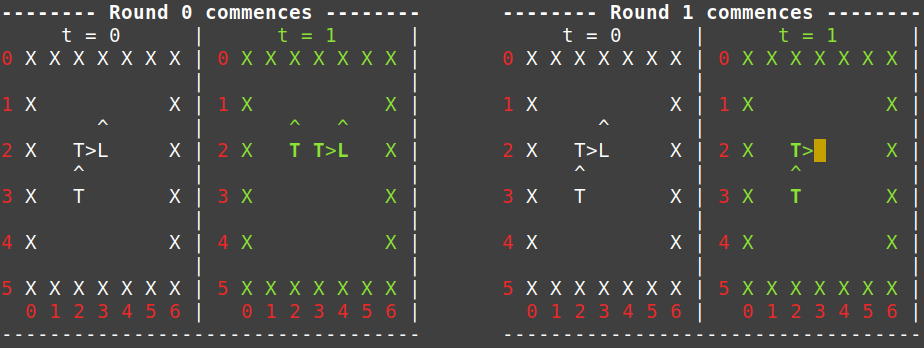
\includegraphics[width=0.75\textwidth]{images/diag_scr_2}
 \caption{In the first round, tanks T at $x=2, y=2$ and $x=2, y=3$ move forward, whilst the tank L at $x=3, y=2$ chooses to wait. As a result, tank L is pushed away. In the second round, the identical scenario plays out, except that a stone (which one is unimportant) chooses to time-jump-in at time $t=1$ onto the square occupied by tank L at time $t=0$. As a result of a time-jump-in onto the waiting tank L, both stones explode and are removed. The time jump still creates an impasse which blocks the movement of tanks T. The game resolves this scenario as follows: 1. The tanks T move forward and the time-jumping stone is placed onto the square which tank L occupies from $t = 0$; 2. A sokoban push is rejected, as the conflicting square is occupied by more than two stones; 3. An impasse reverts the moves of both tanks T; 4. An explosion occurs, destroying both tank L and the time-jumping stone.}\label{fig:scr_2}
\end{center}
\end{figure}
	
	\subsection{Interacting with the past}
	The heart of \textit{Battle of Causality} is time travel. The players are able to perform actions which define a cause and an effect, with the effect happening in an earlier time-slice than the cause. For such an arrangement, we shall use the terms \textbf{ante-effect} and \textbf{retro-cause}.
	
	Naturally, the players cannot \textit{affect} the state of the board in the previous turns or round, only \textit{effect} the state of the board in the next turn, which may happen to correspond to an earlier time. This is why the game is divided into rounds: a \textbf{round} is an interval of assumed consistency, where the game allows players to time-travel as they please, and at the end of each round, \textbf{canonisation} occurs, which ensures the state of the board at the beginning of the next round is "sensible", i.e. causally consistent (see Sec. \ref{sec:canonisation}).
	
	\subsubsection{Canonisation}\label{sec:canonisation}
	Canonisation occurs between every two consecutive rounds. During canonisation, all ante-effects are subject to being activated or deactivated. For each round, the configuration which determines for each ante-effect placed in all \textbf{previous} rounds whether it is active or passive is called a \textbf{scenario}. Canonisation is then, in short, the process of selecting a specific scenario.
	
	For a scenario to be selected, it has to be \textbf{causally consistent}. This means that for every active effect there exists a cause, and every cause has an active effect. Note that for a cause to count, the corresponding flag must be reached and executed by its stone.
	
	\begin{figure}[h]
\begin{center}
    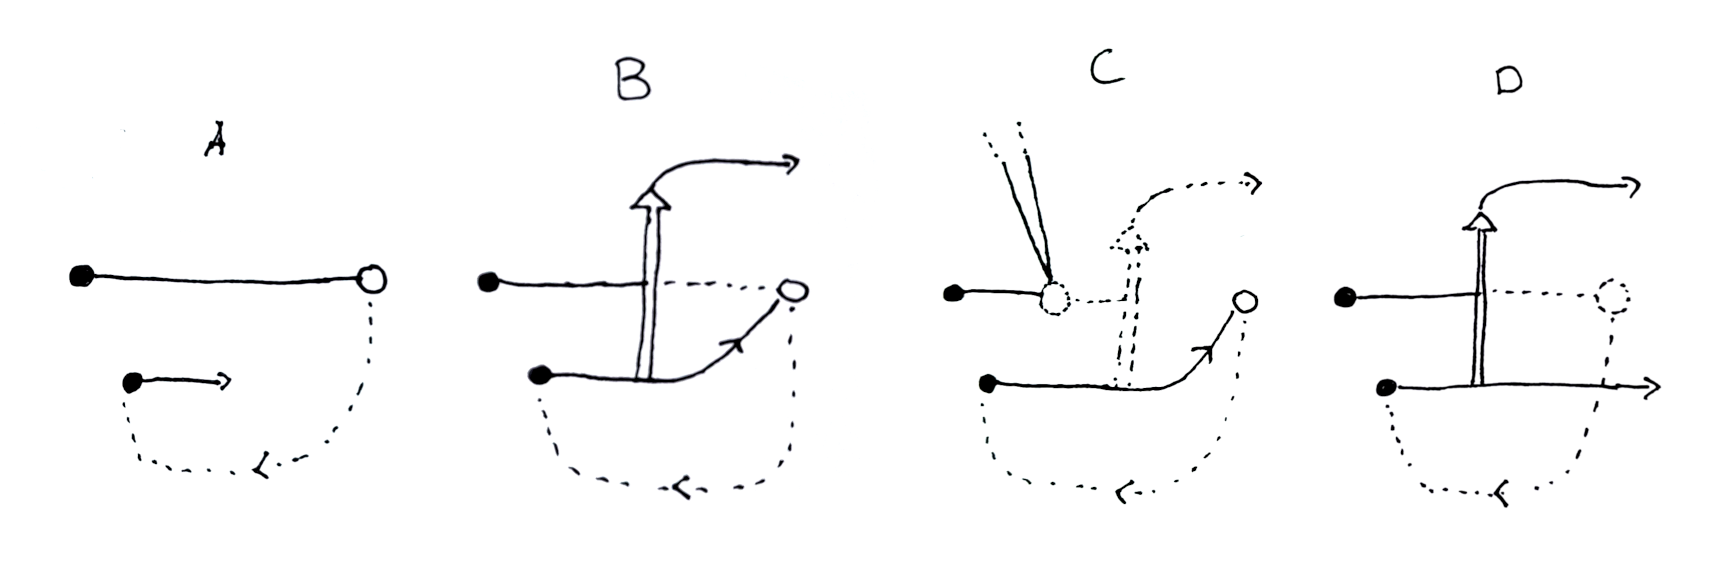
\includegraphics[width=0.85\textwidth]{images/diag_canonisation}
 \caption{In example A, a stone travels back in time, linking the retro-cause (a time-jump-out) to its ante-effect (a time-jump-in). There is only one causally consistent scenario, in which the time-jump-in activates, since the retro-effect is always reached by a stone. In example B, the new version of the stone interferes with its old version, diverting it away from the time-jump-out. However, the new version reaches the time-jump-out and swaps the ante-effect (see below for swapping). There is again only one causally consistent scenario, since deactivating the time-jump-in means the old version of the stone still reaches the time-jump-out. In example C, a new interference destroys the old version of the stone. Here there are two causally consistent scenarios: if the time-jump-in activates, its time-jump-out is reached by the new version, forming a closed worldline. If it deactivates, the time-jump-out is not reached. In example D, the scene from example A continues with the new version interfering with its old version, but not swapping its time-jump-in. Here there are no causally consistent scenarios, since activating the time-jump-in prevents all stones from reaching its time-jump-out, and deactivating it leads to a stone reaching its time-jump-out. A paradox.}\label{fig:canonisation}
\end{center}
\end{figure}
	
	When canonising a round, the game may find one, multiple, or no causally consistent scenarios (for examples, see Fig. \ref{fig:canonisation}). If there exists at least one causally consistent scenario, all candidates are ordered by priority according to specific criterions and the top priority candidate is selected. These criterions can be selected by the players before starting the game, and are further discussed in Sec. \ref{sec:ruleset variations}. If no causally consistent scenarios exist, a paradox is reached. Once again, based on the rules agreed upon by the players, the game may either terminate, or (as per more common rules) attempt to force a causally consistent scenario by deactivating not only player-placed ante-effects, but also the placement of stones on setup. Therefore, a scenario in general entails not only the activity of ante-effects, but also the setup of the first time-slice used for that specific round.
	
	
	\subsubsection{Swapping}\label{sec:swapping}
	Every retro-cause points at one specific ante-effect. However, there isn't a one-to-one relationship, and one ante-effect can admit multiple retro-causes. To \textbf{swap} an ante-effect simply means to add a new retro-cause which links to it, allowing it to be set as active in the next round's scenario in case the swapped retro-cause can activate, too. See Fig. \ref{fig:swapping}.
	
	\begin{figure}[h]
\begin{center}
    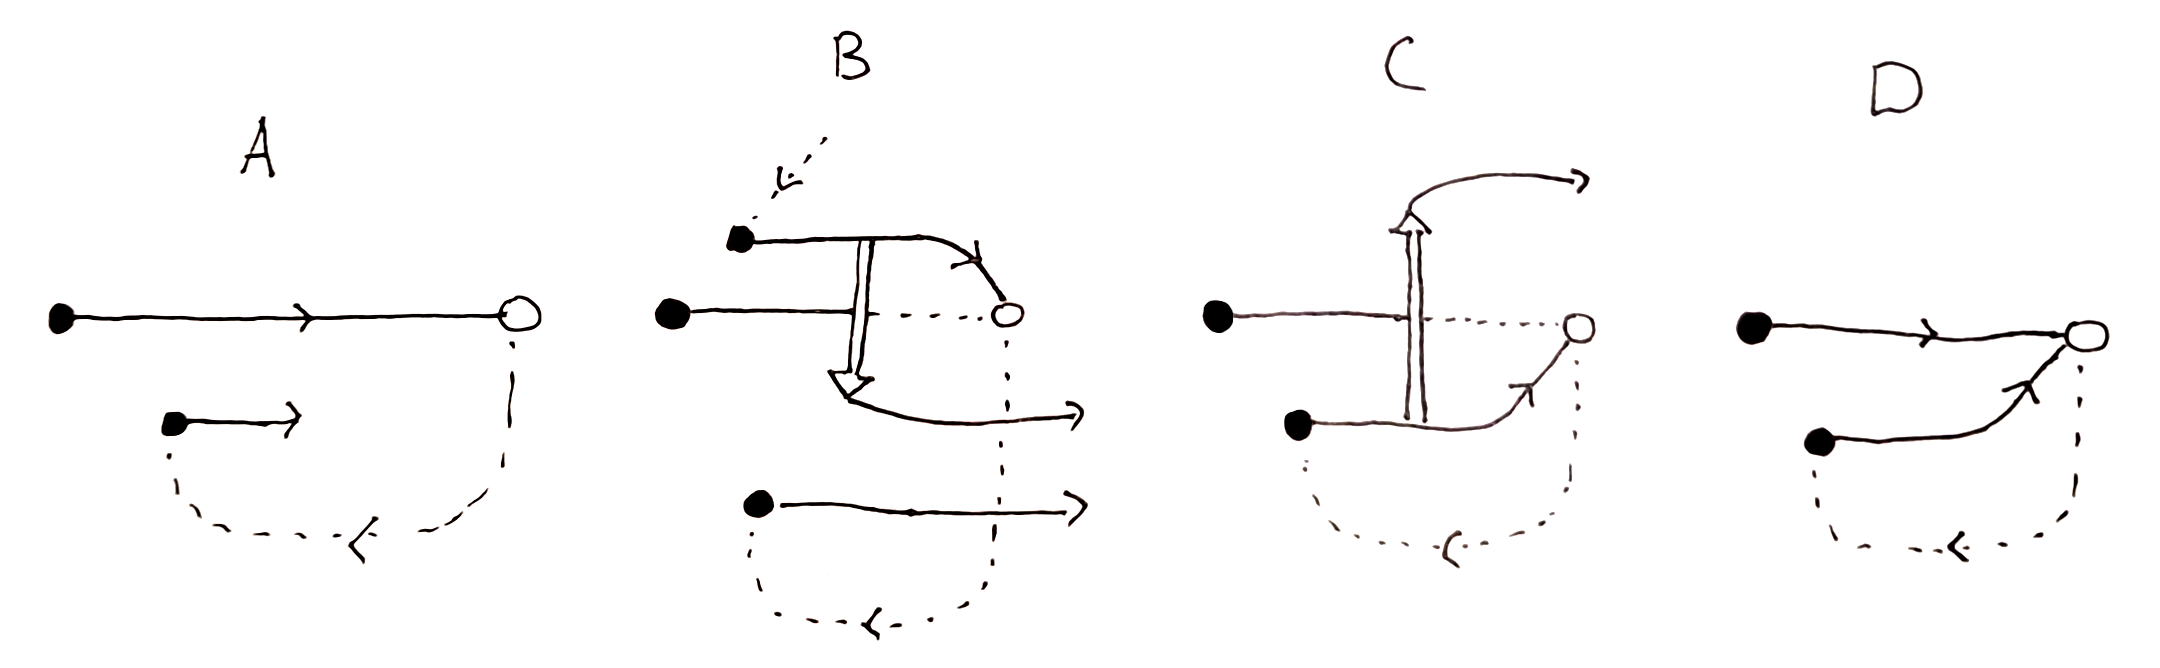
\includegraphics[width=0.9\textwidth]{images/diag_swapping}
 \caption{In example A, a stone travels back in time. The following are three different continuations: in B, a different stone interferes with the old version, preventing its activation of the time-jump-out, but then it swaps the time-jump-in, preserving it as active in the scenario. In C, a similar thing happens, except it is the new version which swaps its own time-jump-in, its worldline forming a closed loop. In D, the new version also swaps its own time-jump-in, but doesn't interfere with the old version. Since there are two activated retro-causes for its time-jump-in, this results in a paradox.}\label{fig:swapping}
\end{center}
\end{figure}

Note that swapping is not mandatory, and a stone which wishes to create a retro-cause linking to an ante-effect on a square which already has an existing ante-effect can choose to create a new ante-effect, for example if the old one will become deactivated anyway. In this sense, swapping is only useful for preserving progenitor ante-effects (namely time-jumps), so that their deactivation doesn't destroy the continuation of a long worldline which passes through them.

	Typically, time-jumps can always be swapped as long as the swapping stone satisfies the conditions of matching stone type, azimuth etc (see Sec. \ref{sec:timejumps}), with the only exception being given by the rule of dogma.
	
	\subsubsection{Rule of dogma}\label{sec:rule of dogma}
	\begin{quote}
	"All ante-effects placed in this round are dogmatic in the next round."
	\end{quote}
	
	Sometimes, placing an ante-effect would result in a paradox or at least its immediate deactivation for the next round. However, if the player gets a bit more leeway, they may be able to justify the ante-effect by swapping it later, or counter-acting the problems it causes with interference. For this reason, \textit{Battle of Causality} makes all ante-effects placed in round $R$ automatically active in round $R+1$. This is an important adjustment to canonisation: during canonisation, the game actually ignores ante-effects placed in this round, only finding a causally consistent scenario for ante-effects placed in all previous rounds (but still taking into account other commands placed in this round, including the newly-placed retro-causes). Then, taking the found scenario, conditions for ending the game are checked, and, if not met, all ante-effects added this round are added to the found scenario as active, and the result is the canonical scenario for the next round. Ante-effects automatically set as active in this way are called dogmatic. For an example, see Fig. \ref{fig:dogma}.
	
	\begin{figure}[h]
\begin{center}
    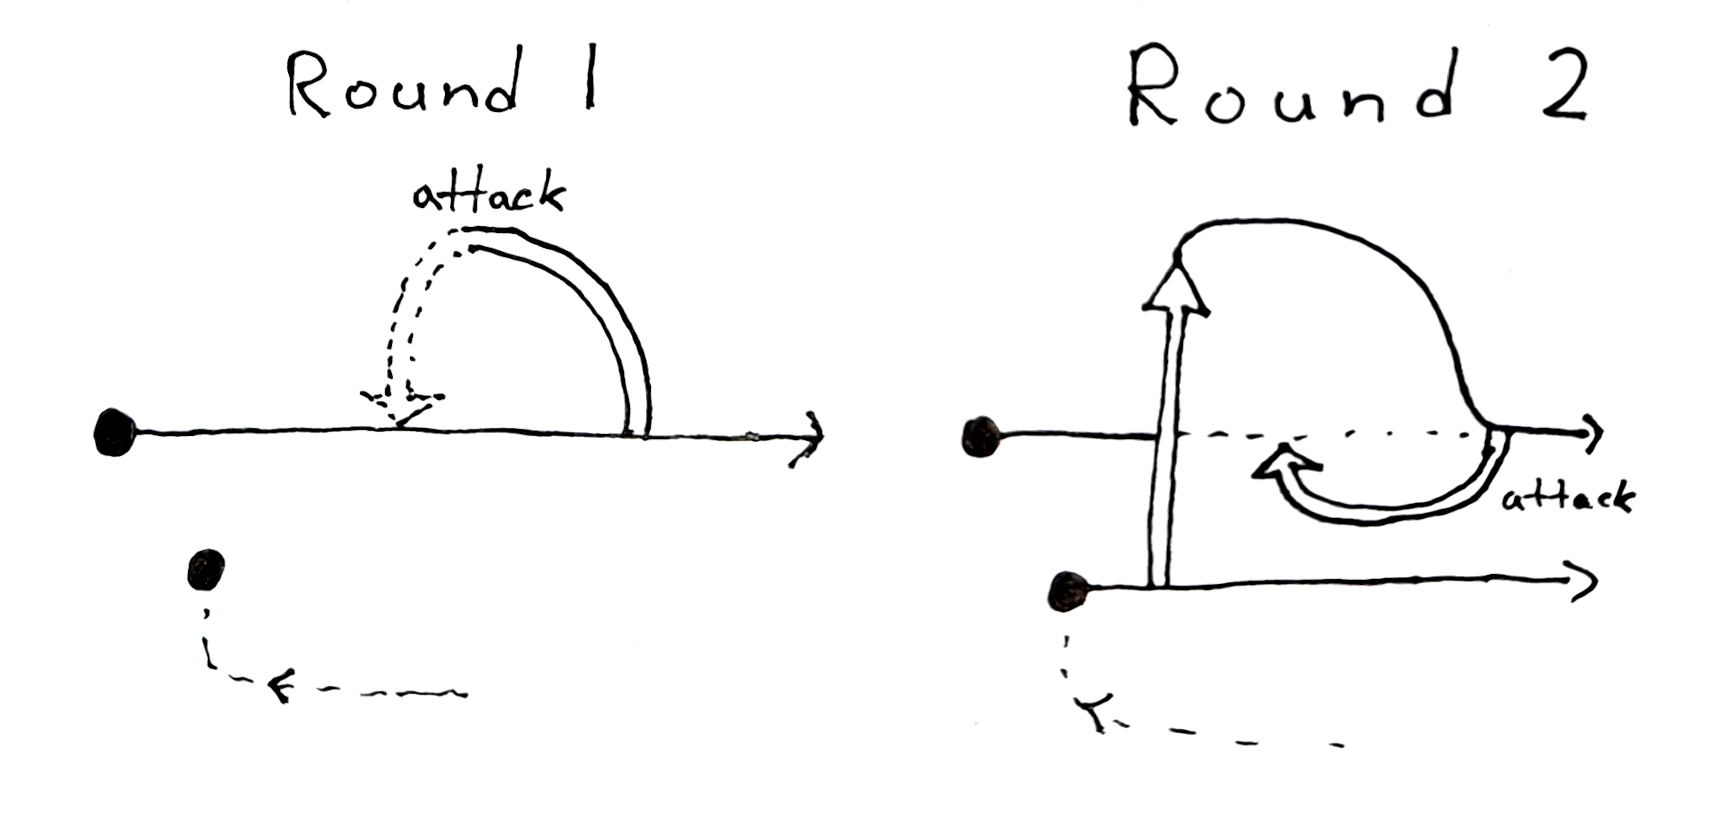
\includegraphics[width=0.6\textwidth]{images/diag_dogma}
 \caption{In round $1$, a bombardier attacks a position in the past, which would destroy the bombardier itself, too. Without the rule of dogma, the existence of the bombardier would be deemed as paradoxical at the end of the round, but thanks to the rule, the ante-effect is preserved as dogmatic in round $2$, although it does not yet have any activated retro-cause. Then, as round $2$ unfolds, a newly placed stone interferes with the bombardier's trajectory, allowing it to dodge its own attack, and later (presumably thanks to the attack) the bombardier is able to return and either swap the attack's ante-effect, or simply create a new attack which performs the same function, making sure the scenario is causally consistent.}\label{fig:dogma}
\end{center}
\end{figure}
	
	Importantly, ante-effects placed in this round cannot be swapped, as that would always result in a paradox. This assures a one-to-one correspondence between ante-effects placed in this round and their retro-causes.
	
	\subsubsection{Time-jumps and other interactions with the past} \label{sec:timejumps}
	The most common way to interact with the past is to take a stone and jump with it to an earlier time-slice. This action is split into two parts: a \textbf{time-jump-out}, which is an action of the old version of the stone, taking it off of the board; and a \textbf{time-jump-in}, a progenitor flag which places the new version of the stone onto the board.
	
	Different stone types can perform time-jumps under different conditions and in different ways which are outlined in Sec. \ref{sec:stone types}. Most importantly, certain stone types are only able to perform a time-jump after reaching the final time-slice of the round, which prevents them from using time-jumps as an easy evasive manoeuver.
	
	Swapping a time-jump-in requires certain conditions to be met. The stones activating the time-jump-in and time-jump-out have to belong to the same faction, be of the same stone-type, and of equal azimuth if orientable. The exception to the latter two conditions is the wildcard, a stone type which can "become" a different stone type by swapping its time-jump-in.
	
	Other ways of interacting with the past are specific to different stone types, and may entail placing bombs at or other forms of attacking a square in a past time-slice. For an exhaustive list, see Sec. \ref{sec:stone types}.
	
	\subsection{End of the game}
	During canonisation, after a causally consistent scenario omitting the recently-added ante-effects is selected, but before the recently-added ante-effects are added as dogmatic, the game finds the state of the board without the dogmatic ante-effects and checks if the conditions for ending the game have been satisfied. There are two classes of game-over conditions: win conditions, which immediately yield the victory to one of the players, and the neutral conditions, which either result in the game counting as a draw, or determining the victor in a different way (see Sec. \ref{sec:ruleset variations} for details).
	
	In the standard game, there is only one win condition: in the canonical scenario, if all bases in the final time-slice belong to a single player, that player wins the game. As mentioned previously, each \textbf{base} corresponds to a stationary spatial position, and the way to conquer it is to visit that position with a stone in one's faction. To be more precise, if a base square is, after spatial conflict resolution, occupied by a stone belonging to a specific player, the base belongs to that player in that and every subsequent timeslice, until it is conquered by another player. Note that if a neutral stone (such as a box or a mine), the allegiance of the base doesn't revert to neutral, but remains as before, since a neutral stone doesn't belong to a specific player.
	
	The win condition can be rephrased as: after selecting the canonical scenario and without applying ante-effects placed in this round, if the last visitor to every base square is a stone belonging to one and the same player, that player wins the game.
	
	As for the neutral conditions, there are a few:
	\begin{enumerate}
		\item "Equilibrium": If, after selecting the canonical scenario, there are no causally free stones in any timeslice (and the win condition remains unsatisfied), the game ends in a draw.
		\item "Stagnation": If no new time-jump-in is placed for three rounds in a row, the game ends in a draw.
	\end{enumerate}
	
	The first condition is straightforward. It can occur if, for example, all causally free stones get destroyed, or if a paradox so unresolvable occurs that the only causally consistent scenario is that in which all stones are removed.

The second condition is also simple, but there's a caveat. Note that if a stone swaps a time-jump-in which would otherwise be deactivated, a new time-jump-out is added, but not a new time-jump-in. Hence, a non-swapping time-jump has to be executed at least every third round. Note that time-jumps-in do not have to be placed in order to avoid triggering the "Equilibrium" condition: an intricate dynamic of activating and deactivating time-jumps-in through causal consistency selection may assure the presence of at least a handful of causally-free stones on the board in each round. However, if no new time-jumps-in are placed for a long time, and the win condition remains unsatisfied, it is assumed that the game degenerated into a fruitless back-and-forth, and is terminated. This condition also maintains a sense of pacing in the game, as adding more and more time-jumps-in makes the game more and more unstable (in the sense that the number of possible scenarios grows, and so larger and larger sets of activations and deactivations may occur at the end of each round), threatening to tip off the first condition.
	
	
	\section{Stone types}\label{sec:stone types}
	There are multiple types of stones, a multitude of which may be at each player's disposal throughout the game. These stones differ in their ways of moving, attacking, time-jumping etc. The following is a list of the stone types currently in the game\footnote{The game is open-source, and I encourage you all to add all the new stone types you can think of!}:
	\begin{itemize}
	\item \textbf{Tank}
		\begin{itemize}
		\item Opposable
		\item Orientable
		\item Movement: the tank can move forwards or backwards by 1 square and then optionally turn clockwise or anticlockwise by a quarter-revolution. Alternatively, it can stay on its square and turn to any azimuth, or remain as it is.
		\item Attacking: the tank attacks by firing in the direction of its azimuth, destroying the first stone in its line of sight, regardless of the stone's faction.
		\item Time-jumps: the tank can only time-jump after reaching the final time-slice.
		\end{itemize}
	\item \textbf{Bombardier}
		\begin{itemize}
		\item Opposable
		\item Unorientable
		\item Movement: the bombardier can move by $1$ square in each of the $4$ cardinal directions.
		\item Attacking: the bombardier attacks by dropping a bomb onto the same spatial position in any previous time-slice. Being an ante-effect, the consequences of the attack don't unfold until the next round. The bomb destroys any stone on the target square and all of the $4$ adjanced squares.
		\item Time-jumps: the bombardier can only time-jump after reaching the final time-slice.
		\end{itemize}
	\item \textbf{Sniper}
		\begin{itemize}
		\item Opposable
		\item Orientable
		\item Movement: the sniper cannot move on its own, and relies on being pushed by other opposable stones. However, it can turn to any azimuth or remain as it is.
		\item Attacking: the sniper attacks by firing in the direction of its azimuth, destroying the first stone in its line of sight except for stones in the same faction. Stones in the same faction are ignored and the attack can hit even stones obscured behind them.
		\item Time-jumps: the sniper can time-jump from any time-slice into any previous time-slice.
		\end{itemize}
	\item \textbf{Tagger}
		\begin{itemize}
		\item Unopposable
		\item Unorientable
		\item Movement: the tagger jumps like a horse (two squares in any cardinal direction and one square in a perpendicular direction). Being unopposable, it naturally jumps over other stones.
		\item Attacking: the tagger deploys a tagscreen at its position, tagging any stone on its square and all of the $4$ adjanced squares. There are multiple different tagscreen types the player can choose from:
		\begin{itemize}
			\item "Lock" tagscreen: The tagged stones lose their ability to time-jump-out and become causally locked in the final time-slice. However, this does not disrupt time-jumps-out already placed on the tagged stones' trajectories, only prevents the players for queueing new ones.
			\item "Unlock" tagscreen: counteracts the "lock" tagscreen, or interferes with trajectories laid out on previous rounds, making stones causally free. See Sec. \ref{sec:ruleset variations} for details.
			\item "Hide" tagscreen: Removes all tagged stones from the board and places them into the next time-slice. Cannot be deployed on the second-to-last time-slice.
		\end{itemize}
		\item Time-jumps: the tagger can time-jump at any time, but its time-jumps still obey the rules of its movement--either by two time-slices back and by one square in any cardinal direction, or by one time-slice back and by two squares in any cardinal direction.
		\end{itemize}
	\item \textbf{Wildcard}
		\begin{itemize}
		\item Unopposable
		\item Unorientable
		\item Movement: the wildcard jumps onto the neighbouring square in any of the $4$ diagonal directions.
		\item Attacking: the wildcard attacks on movement, destroying all stones sharing its square right before spatial conflict resolution, akin to captures in chess. Two or more wildcards can capture each other, destroying all stones present. The wildcard does not capture a stone which jumps onto its square if waiting.
		\item Time-jumps: the wildcard can time-jump at any time. A special property of the wildcard is that it can swap the time-jump of any stone type (and is not limited by the azimuth if changing into an orientable stone). For more details on swapping, see Sec. \ref{sec:swapping}.
		\item The wildcard cannot capture bases.
		\end{itemize}
	\end{itemize}
	There are also neutral stones, which are not controlled by any player, and are simply placed onto the board to be interacted with:
	\begin{itemize}
		\item \textbf{Box}: an unorientable stone which can be pushed around. It is destroyed if targeted by an attack.
		\item \textbf{Mine}: an unorientable stone. If a stone ends up on the same square as a mine after flag execution but \textit{before} spatial conflict resolution, instead of the mine being pushed or the stone returning back, there is an explosion which destroyes all stones on this and the four adjanced squares. Note that because this overrides spatial conflict resolution, the \textbf{impasse} rule doesn't prevent multiple stones from stepping onto the mine and exploding all together!
	\end{itemize}
	
	\section{Ruleset variations}\label{sec:ruleset variations}
	There are multiple aspects of the game where game behaviour can be customised by the players by agreement before the game begins. These customisations are realised as a lists of behaviour characteristics, where for each list, one option has to be selected. The following ruleset variations are currently implemented in the game:
	\begin{enumerate}
		\item Reaching a paradox (a situation where no possible scenario for the next round is causally consistent) results in what action?
		\begin{enumerate}
			\item "Auditors of Reality": Variations of deactivating stones on setup are tried in a specific order (prioritizing an arbitrary ordering, see below) until a causally-consistent scenario is possible. Setup stones deactivated this way stay deactivated for the rest of the game, even if, in future canonizations, their reactivation would be causally consistent.
			\item "Hulot's Holiday": Same as 'Auditors of reality', except the stones are not removed permanently and their reactivation is considered in every future canonization.
			\item "Know your paradoxes!": A paradox immediately ends the game!
		\end{enumerate}
		\item If the game ends with no players satisfying the primary win condition, what is the outcome of the game?
		\begin{enumerate}
			\item "Poiccard's Gambit": The game counts as a draw.
			\item "Fighting in the War Room": If one player owns the majority of bases in the final timeslice of the last canonized round, that player wins the game.
		\end{enumerate}
		\item If two or more scenarios are possible during canonisation, which one is selected? (The following are ordered lists of criterions, where the candidates will be ordered by the first criterion, then the second etc. until there is only one with top priority.)
		\begin{enumerate}
			\item "Shield and Spear":
			\begin{enumerate}
				\item Smaller number of setup deactivations is prioritized
				\item Not deactivating setup stones more recently touched by the player is prioritized
				\item Activating ante-effects added more recently is prioritized
			\end{enumerate}
			\item "Ace Wildcard":
			\begin{enumerate}
				\item Not deactivating stones (setup or time-jumped-in) more recently touched by the player is prioritized
				\item Activating ante-effects added more recently is prioritized
			\end{enumerate}
			\item "Merry Chronos":
			\begin{enumerate}
				\item Bigger number of active ante-effects is prioritized
				\item Bigger number of stones present on board is prioritized
				\item Keeping more recently added stones is prioritized (where the recency of setup stones is determined in first round by a headcount by each player)
				\item Activating ante-effects added more recently is prioritized
			\end{enumerate}
		\end{enumerate}
		If "Know your paradoxes!" is selected and therefore the game does not permit deactivating setup stones, the following two options are instead available:
		\begin{enumerate}
			\item "Out with the Old": Activating ante-effects added more recently is prioritized
			\item "Conservative":
			\begin{enumerate}
				\item Bigger number of active ante-effects is prioritized
				\item Activating ante-effects added more recently is prioritized
			\end{enumerate}
		\end{enumerate}
		\item On a turn with active time-slice $t$, can the players view the entire board?
		\begin{enumerate}
			\item "Omniscience": The players can view the entire board, informing them of all ante-effects placed by the other player.
			\item "Fog of War": The players cannot view time-slices $t+1,t+2\dots t_{\text{time cap}}$. This means the players learn of the other player's recently placed ante-effects as they progress through the round where these ante-effects manifest for the first time. However, the players can still view the canonised version of the round which omits the dogmatic ante-effects.
		\end{enumerate}
	\end{enumerate}
	
	Extra explanation is needed for the rules concerned with assigning priorities to scenarios based on deactivating setup stones.
	
	A stone is "touched" by a player when a command is submitted for it, changing the position on which it is causally free. The order of touch recency is firstly turn-by-turn, but also within each turn, and so the game may behave differently depending on what order one submits commands for their causally free stones in a single turn.
	
	A "headcount" is an action which, if required by the rules, is performed by the players at the start of the game once. It is a method of assigning recency of placement to progenitor flags which are placed automatically during the stup of the game.
	
	For both of these recency orderings, an extra assymetry enters between the players. Since both players submit their actions for each turn simultaneously, and their stones are placed onto the board on setup simultaneously, an arbitrary tie-breaker is created like so: if player $A$ submits two commands for their two causally free stones $A_1,A_2$ in this order, and player $B$ submits three commands for their three causally free stones $B_1, B_2, B_3$ in this order, the total recency ordering for these stones is a "zig-zag stitch" between the two sub-sequences, beginning with player $A$; in this case, the recency ordering of touch would be $A_1,B_1,A_2,B_2,B_3$. The same works for headcounts: both players submit their headcounts, and the final recency ordering is the same zig-zag stitch, starting with $A$. This means that the game treats players $A$ and $B$ asymmetrically, although player $A$'s advantage is significantly smaller than, say, the advantage white has in chess.
	
	\section{Glossary}
{\renewcommand{\arraystretch}{0.5}
 \begin{longtable}{ R{0.15\linewidth}  L{0.81\linewidth}  }

\rowlabel{glossary:active} \\* \textbf{active} & \parbox[t]{\linewidth}{This term may depend mulitple things depending on the context. A flag is said to be active if its activity has been set as such in a scenario. A time-slice is said to be active in every turn in which the players are prompted to command their stones in that time-slice. See \hyperref[glossary:activity]{\textbf{activity}}, \hyperref[glossary:turn]{\textbf{turn}}.}\\
\rowlabel{glossary:activity} \\* \textbf{activity} & \parbox[t]{\linewidth}{A flag can be set as active or passive. An active flag behaves normally. A passive flag is ignored by the stone it's attached to, and the stone behaves as if the flag was not placed at all. See \hyperref[glossary:flag]{\textbf{flag}}, \hyperref[glossary:active]{\textbf{active}}.}\\
\rowlabel{glossary:allegiance} \\* \textbf{allegiance} & \parbox[t]{\linewidth}{A property of a base, determining the last faction which conquered that base, or "neutral" if determined as such on setup. See \hyperref[glossary:faction]{\textbf{faction}}.}\\
\rowlabel{glossary:ante-effect} \\* \textbf{ante-effect} & \parbox[t]{\linewidth}{An effect that precedes its cause on the time-axis. See \hyperref[glossary:retro-cause]{\textbf{retro-cause}}.}\\
\rowlabel{glossary:azimuth} \\* \textbf{azimuth} & \parbox[t]{\linewidth}{The orientation of an orientable stone, which can be up (negative $y$ direction), right (positive $x$ direction), down (positive $y$ direction), or left (negative $x$ direction). See \hyperref[glossary:orientable]{\textbf{orientable}}.}\\
\rowlabel{glossary:base} \\* \textbf{base} & \parbox[t]{\linewidth}{A square which can be captured by a player visiting it with one of their stones, and it remains captured until their opponent visits it themselves. The goal of the game is to reach a scenario where all the bases end up captured by your stones in the final time-slice. See \hyperref[glossary:allegiance]{\textbf{allegiance}}.}\\
\rowlabel{glossary:canon} \\* \textbf{canon} & \parbox[t]{\linewidth}{The canon of the board is its evolution throughout the turns of the game. Even though time may go back, turns always progress forward, and once the state of the board for a specific turn has been determined, it cannot change again--we say it is canonical. A canonical state cannot be conflicting. See \hyperref[glossary:conflicting]{\textbf{conflicting}}.}\\
\rowlabel{glossary:canonisation} \\* \textbf{canonisation} & \parbox[t]{\linewidth}{At the end of each round, the highest-priority causally consistent scenario is selected for the next round based on the flags placed so far, omitting ante-effects placed in the round which just ended. See \hyperref[glossary:causally consistent]{\textbf{causally consistent}}.}\\
\rowlabel{glossary:causally consistent} \\* \textbf{causally consistent} & \parbox[t]{\linewidth}{Not resulting in a paradox. See \hyperref[glossary:scenario]{\textbf{scenario}}, \hyperref[glossary:paradox]{\textbf{paradox}}.}\\
\rowlabel{glossary:causally free} \\* \textbf{causally free} & \parbox[t]{\linewidth}{A stone is causally free at a specific position if it is placed on the board at that position, but is not subject to a flag at that position.}\\
\rowlabel{glossary:causally locked} \\* \textbf{causally locked} & \parbox[t]{\linewidth}{Present on the board, but not causally free. See \hyperref[glossary:causally free]{\textbf{causally free}}.}\\
\rowlabel{glossary:comb rule} \\* \textbf{comb rule} & \parbox[t]{\linewidth}{The comb rule states that for each turn there may be no causally free stones in time-slices preceding the active time-slice. Therefore, for all but the final time-slice each player must command all of their causally free stones.}\\
\rowlabel{glossary:conflicting} \\* \textbf{conflicting} & \parbox[t]{\linewidth}{Not adhering to the rules which specify what the board can and cannot look like. Typically, the movement of stones in each turn sends them into conflicting positions, which are subsequently resolved by the game to find the canonical state of the next time-slice. See \hyperref[glossary:canon]{\textbf{canon}}.}\\
\rowlabel{glossary:dogma} \\* \textbf{dogma} & \parbox[t]{\linewidth}{A flag is said to be dogmatic in a specific round if it is set as active in the round's scenario due to a special rule (the \hyperref[sec:rule of dogma]{rule of dogma}), not because it was set as active due to the selection of a high-priority causally consistent scenario. See \hyperref[glossary:rule of dogma]{\textbf{rule of dogma}}.}\\
\rowlabel{glossary:faction} \\* \textbf{faction} & \parbox[t]{\linewidth}{A player; i.e. "this stone's faction" synonymous to "the player this stone belongs to".}\\
\rowlabel{glossary:flag} \\* \textbf{flag} & \parbox[t]{\linewidth}{A command placed at a specific position, for a specific stone, by the player. Flags can order the stones to attack, move, time-jump etc.}\\
\rowlabel{glossary:interference} \\* \textbf{interference} & \parbox[t]{\linewidth}{The act of obstructing the trajectory of a stone established in previous rounds. This makes the stone causally free again, but can also prevent it from activating its associated retro-causes.}\\
\rowlabel{glossary:opposable} \\* \textbf{opposable} & \parbox[t]{\linewidth}{If a stone is opposable, then it moves in a way which allows it to push other stones, but its movement can also be blocked by a stone moving in the opposite direction. See \hyperref[glossary:unopposable]{\textbf{unopposable}}.}\\
\rowlabel{glossary:orientable} \\* \textbf{orientable} & \parbox[t]{\linewidth}{If a stone is orientable, then its trajectory is described not only by its positions, but also their corresponding azimuths. Orientable stones move and attack in ways which depend on their azimuth. See \hyperref[glossary:azimuth]{\textbf{azimuth}}.}\\
\rowlabel{glossary:paradox} \\* \textbf{paradox} & \parbox[t]{\linewidth}{A scenario such that if we evolve the board along the time axis, there will either be active ante-effects which have zero or multiple activated retro-causes, or activated retro-causes which correspond to an inactive ante-effect.}\\
\rowlabel{glossary:position} \\* \textbf{position} & \parbox[t]{\linewidth}{One square on the board in one specific time-slice. Parametrised by three numbers: (t, x, y). See \hyperref[glossary:spatial position]{\textbf{spatial position}}, \hyperref[glossary:causally free]{\textbf{causally free}}.}\\
\rowlabel{glossary:precede} \\* \textbf{precede} & \parbox[t]{\linewidth}{Occur in a time-slice with time smaller than}\\
\rowlabel{glossary:priority} \\* \textbf{priority} & \parbox[t]{\linewidth}{Every scenario has a priority. If two or more scenarios are causally consistent for a round, the one with highest priority is canonised. See \hyperref[glossary:scenario]{\textbf{scenario}}, \hyperref[glossary:canonisation]{\textbf{canonisation}}.}\\
\rowlabel{glossary:progenitor} \\* \textbf{progenitor} & \parbox[t]{\linewidth}{A progenitor is a flag which, when active, places a new stone onto its associated position. Progenitors are unique in the way that they are associated with a specific stone, but do not require the presence of that stone at their position to be activated--rather, when activated, they place the stone themselves.}\\
\rowlabel{glossary:recency} \\* \textbf{recency} & \parbox[t]{\linewidth}{A property of ante-effects and stones, determined depending on the specific ruleset (see Sec. \ref{sec:ruleset variations}). Stones and ante-effects with higher recency are more likely to be preserved during canonisation if two or more causally consistent scenarios are possible.}\\
\rowlabel{glossary:retro-cause} \\* \textbf{retro-cause} & \parbox[t]{\linewidth}{A cause that occurs after its effect on the time-axis. We say that a retro-cause is \textit{activated} if it is executed by its corresponding stone at its position in some specific scenario. See \hyperref[glossary:ante-effect]{\textbf{ante-effect}}.}\\
\rowlabel{glossary:round} \\* \textbf{round} & \parbox[t]{\linewidth}{The progress of the game occurs in rounds. In each round, players command their stones for every time-slice with increasing time, and after reaching the end, the round is canonised. See \hyperref[glossary:turn]{\textbf{turn}}, \hyperref[glossary:canonisation]{\textbf{canonisation}}.}\\
\rowlabel{glossary:rule of dogma} \\* \textbf{rule of dogma} & \parbox[t]{\linewidth}{All ante-effects placed in this round are dogmatic in the next round. See \hyperref[glossary:dogma]{\textbf{dogma}}.}\\
\rowlabel{glossary:scenario} \\* \textbf{scenario} & \parbox[t]{\linewidth}{A scenario for a given round specifies which ante-effects placed in all the previous rounds are active and which are passive in that round, and which setup placements are omitted. See \hyperref[glossary:activity]{\textbf{activity}}, \hyperref[glossary:setup]{\textbf{setup}}.}\\
\rowlabel{glossary:setup} \\* \textbf{setup} & \parbox[t]{\linewidth}{A set of progenitors which place stones on the board in the first time-slice. See \hyperref[glossary:progenitor]{\textbf{progenitor}}.}\\
\rowlabel{glossary:spatial position} \\* \textbf{spatial position} & \parbox[t]{\linewidth}{One square on the board across all time-slices. Parametrised by two numbers: (x, y). See \hyperref[glossary:position]{\textbf{position}}.}\\
\rowlabel{glossary:stone} \\* \textbf{stone} & \parbox[t]{\linewidth}{A stone is a unit which belongs to a player and is commanded by them, or is neutral (for example a box or a mine). The term \textbf{stone} implies continuity across time-slices but not across time-jumps. In other words, if a stone is placed on the board in the first time-slice and then makes a series of spatial moves, which propagate it into the final time-slice, we say it is still the same stone; however, if that stone then jumps back in time into the first time-slice, we say that the stone placed in the first time-slice is another, new stone. See \hyperref[glossary:worldline]{\textbf{worldline}}.}\\
\rowlabel{glossary:swap} \\* \textbf{swap} & \parbox[t]{\linewidth}{To swap an ante-effect means to add a new retro-cause to it, which can prevent its deactivation during subsequent canonisations, but can also result in a paradox if the number of retro-causes becomes too big. See \hyperref[glossary:paradox]{\textbf{paradox}}.}\\
\rowlabel{glossary:time} \\* \textbf{time} & \parbox[t]{\linewidth}{An axis on the board, akin to horizontal and vertical position.}\\
\rowlabel{glossary:time cap} \\* \textbf{time cap} & \parbox[t]{\linewidth}{The length of the time axis. The value of time runs from $0$ to $(\text{time cap}) - 1$.}\\
\rowlabel{glossary:time-jump} \\* \textbf{time-jump} & \parbox[t]{\linewidth}{The act of jumping back in time. For every stone, there will be opportunity to make a time-jump and re-join the game in the next round, when the earlier time-slices become available to place flags in once again.}\\
\rowlabel{glossary:time-slice} \\* \textbf{time-slice} & \parbox[t]{\linewidth}{A section of the board specified by a given value of time. Analogous to "rank" and "file" for horizontal and vertical position in chess.}\\
\rowlabel{glossary:trajectory} \\* \textbf{trajectory} & \parbox[t]{\linewidth}{The set of positions along the time axis of a stone from the time when it was placed on the board until the time it was removed from the board, or became causally free.}\\
\rowlabel{glossary:turn} \\* \textbf{turn} & \parbox[t]{\linewidth}{Every round is divided into a number of turns equal to the time cap. Each turn corresponds to one time-slice (the \textbf{active} time-slice), and in each turn every player places down flags for their causally free stones in that time-slice. See \hyperref[glossary:round]{\textbf{round}}, \hyperref[glossary:active]{\textbf{active}}.}\\
\rowlabel{glossary:unopposable} \\* \textbf{unopposable} & \parbox[t]{\linewidth}{If a stone is unopposable, then it essentially jumps over other stones, and thus cannot be blocked by a stone moving in the opposite direction. However, such a stone's movement is always blocked when it attempts to jump onto an occupied square, since it is unable to push other stones. See \hyperref[glossary:opposable]{\textbf{opposable}}.}\\
\rowlabel{glossary:unorientable} \\* \textbf{unorientable} & \parbox[t]{\linewidth}{If a stone is unorientable, then its trajectory is described only by its positions. The movement and attack pattern of unorientable stones is symmetric under rotation by a quarter-revolution. See \hyperref[glossary:orientable]{\textbf{orientable}}.}\\
\rowlabel{glossary:worldline} \\* \textbf{worldline} & \parbox[t]{\linewidth}{A worldline is a collection of trajectories belonging to a sequence of stones where each stone ends their trajectory by a time-jump which creates the next stone. A worldline can change its structure as the game progresses, by interference and swapping. See \hyperref[glossary:trajectory]{\textbf{trajectory}}, \hyperref[glossary:swap]{\textbf{swap}}.}


\end{longtable}}
	
	
	
	
	
	

	
	
\end{document}
